\begin{center}

\includegraphics[width=0.4\textwidth]{content/3/chapter5/images/18.png}\\
Cippi studies the calendar
\end{center}

\begin{tcolorbox}[colback=blue!5!white,colframe=blue!75!black,title={Lack of Compiler Support}]
	
At the end of 2020, no C++ compiler supports the chrono extensions so far. Thanks to the prototype library \href{https://github.com/HowardHinnant/date}{date} from Howard Hinnant, which is essentially a superset of the extended time functionality in C++20, I can experiment with it. The library is hosted on GitHub. There are various ways to use the date prototype:

\begin{itemize}
\item 
You can try it out on Wandbox. Howard has uploaded the date.h header, which is sufficient to play with the new type std::time\_of\_day and the calendar. Here is Howard’s link: \href{https://wandbox.org/permlink/L8MwjzSSC3fXXrMd}{Try it out on Wandbox!}.

\item 
Download the project and build it. The already mentioned GitHub page \href{https://github.com/HowardHinnant/date}{date} gives you more information. This step is required when you want to try out the new time zone features.
\end{itemize}

The examples in this chapter use Howard Hinnant’s library. My explanations, though, are based on the C++20 terminology. When a C++ compiler supports the extended chrono functionality, I will adapt the examples to the C++20 syntax.

\end{tcolorbox}

\begin{itemize}
\item 
The time of day is the time duration since midnight, split into hours, minutes, seconds, and fractional seconds.

\item 
Calendar stands for various calendar dates such as year, a month, a weekday, or the n-th day of a week.

\item 
A time zone represents time specific to a geographic area.
\end{itemize}

Essentially, the time-zone functionality (C++20) is based on the calendar functionality (C++20), and the calendar functionality (C++20) is based on the chrono functionality (C++11).


\begin{tcolorbox}[colback=blue!5!white,colframe=blue!75!black,title={Lack of Compiler Support}]
	
To get the most out of this section, a basic understanding of the chrono library is essential.
C++11 introduced three main components to deal with time:

\begin{itemize}
\item 
A time point is defined by a starting point, the so-called epoch, and additional time duration.

\item 
A time duration is the difference between two time points. It is given by the number of ticks.

\item 
A clock consists of a starting point (epoch) and a tick, so that the current time point can be calculated.
\end{itemize}

Honestly, time, for me, is a mystery. On one hand, each of us has an intuitive idea of time, on the other hand, defining it formally is extremely challenging. For example, the three components time point, time duration, and clock depend on each other. If you want to know more about the time functionality in C++11, read my posts about time from \href{https://www.modernescpp.com/index.php/tag/time}{time}.
	
\end{tcolorbox}

\subsubsubsection{5.5.1\hspace{0.2cm} Time of day}

std::chrono::hh\_mm\_ss is the duration since midnight, split into hours, minutes, seconds, and fractional seconds. This type is typically used as a formatting tool. First, the following table gives you a concise overview of std::chrono::hh\_mm\_ss instance tOfDay.

\begin{center}
Time of Day
\end{center}

\begin{table}[H]
\centering
\begin{tabular}{ll}
\textbf{Function}         & \textbf{Description}                        \\ \hline
tOfDay.hours()            & Returns the hour component since midnight   \\
tOfDay.minutes()          & Returns the minute component since midnight \\
tOfDay.seconds()          & Returns the second component since midnight \\
tOfDay.subseconds()       & Returns the fractional second component since midnight  \\
tOfDay.to\_duration()     & Returns the time duration since midnight    \\
std::chrono::make12(hour) & Returns the 12-hour equivalent of a 24-hour format time \\
std::chrono::make12(hour  & Returns the 24-hour equivalent of a 12-hour format time \\
std::chrono::is\_am(hour) & Detects if the 24-hour format time is a.m.  \\
std::chrono::is\_pm(hour) & Detects if the 24-hour format time is p.m. 
\end{tabular}
\end{table}


he use of the functions is straightforward.

\hspace*{\fill} \\ %插入空行
\noindent
Time of day
\begin{lstlisting}[style=styleCXX]
// timeOfDay.cpp

#include "date.h"
#include <iostream>

int main() {
	using namespace date;    \
	
	using namespace std::chrono_literals;
	
	std::cout << std::boolalpha << '\n';
	auto timeOfDay = date::hh_mm_ss(10.5h + 98min + 2020s + 0.5s);
	
	std::cout<< "timeOfDay: " << timeOfDay << '\n';
	
	std::cout << '\n';
	
	std::cout << "timeOfDay.hours(): " << timeOfDay.hours() << '\n';
	std::cout << "timeOfDay.minutes(): " << timeOfDay.minutes() << '\n';
	std::cout << "timeOfDay.seconds(): " << timeOfDay.seconds() << '\n';
	std::cout << "timeOfDay.subseconds(): " << timeOfDay.subseconds() << '\n';
	std::cout << "timeOfDay.to_duration(): " << timeOfDay.to_duration() << '\n';
	std::cout << '\n';
	
	std::cout << "date::hh_mm_ss(45700.5s): " << date::hh_mm_ss(45700.5s) << '\n';
	
	std::cout << '\n';
	
	std::cout << "date::is_am(5h): " << date::is_am(5h) << '\n';
	std::cout << "date::is_am(15h): " << date::is_am(15h) << '\n';
	
	std::cout << '\n';
	
	std::cout << "date::make12(5h): " << date::make12(5h) << '\n';
	std::cout << "date::make12(15h): " << date::make12(15h) << '\n';

}
\end{lstlisting}

First, I create in line 12 a new instance of std::chrono::hh\_mm\_ss: timeOfDay. Thanks to the chrono literals from C++14, I can add a few time durations to initialize a time of day object. With C++20, you can directly output timeOfDay (line 14). This is the reason I have to introduce the namespace date in line 7. The rest should be straightforward to read. Lines 18 - 21 display the components of the time since midnight in hours, minutes, seconds, and fractional seconds. Line 22 returns the time duration since midnight in seconds. Line 26 is more interesting: the given seconds correspond to the time displayed in line 15. Lines 30 and 32 return if the given hour is a.m. Line 35 and 36 return the 12-hour equivalent of the given hour.

Here is the output of the program:

\begin{center}
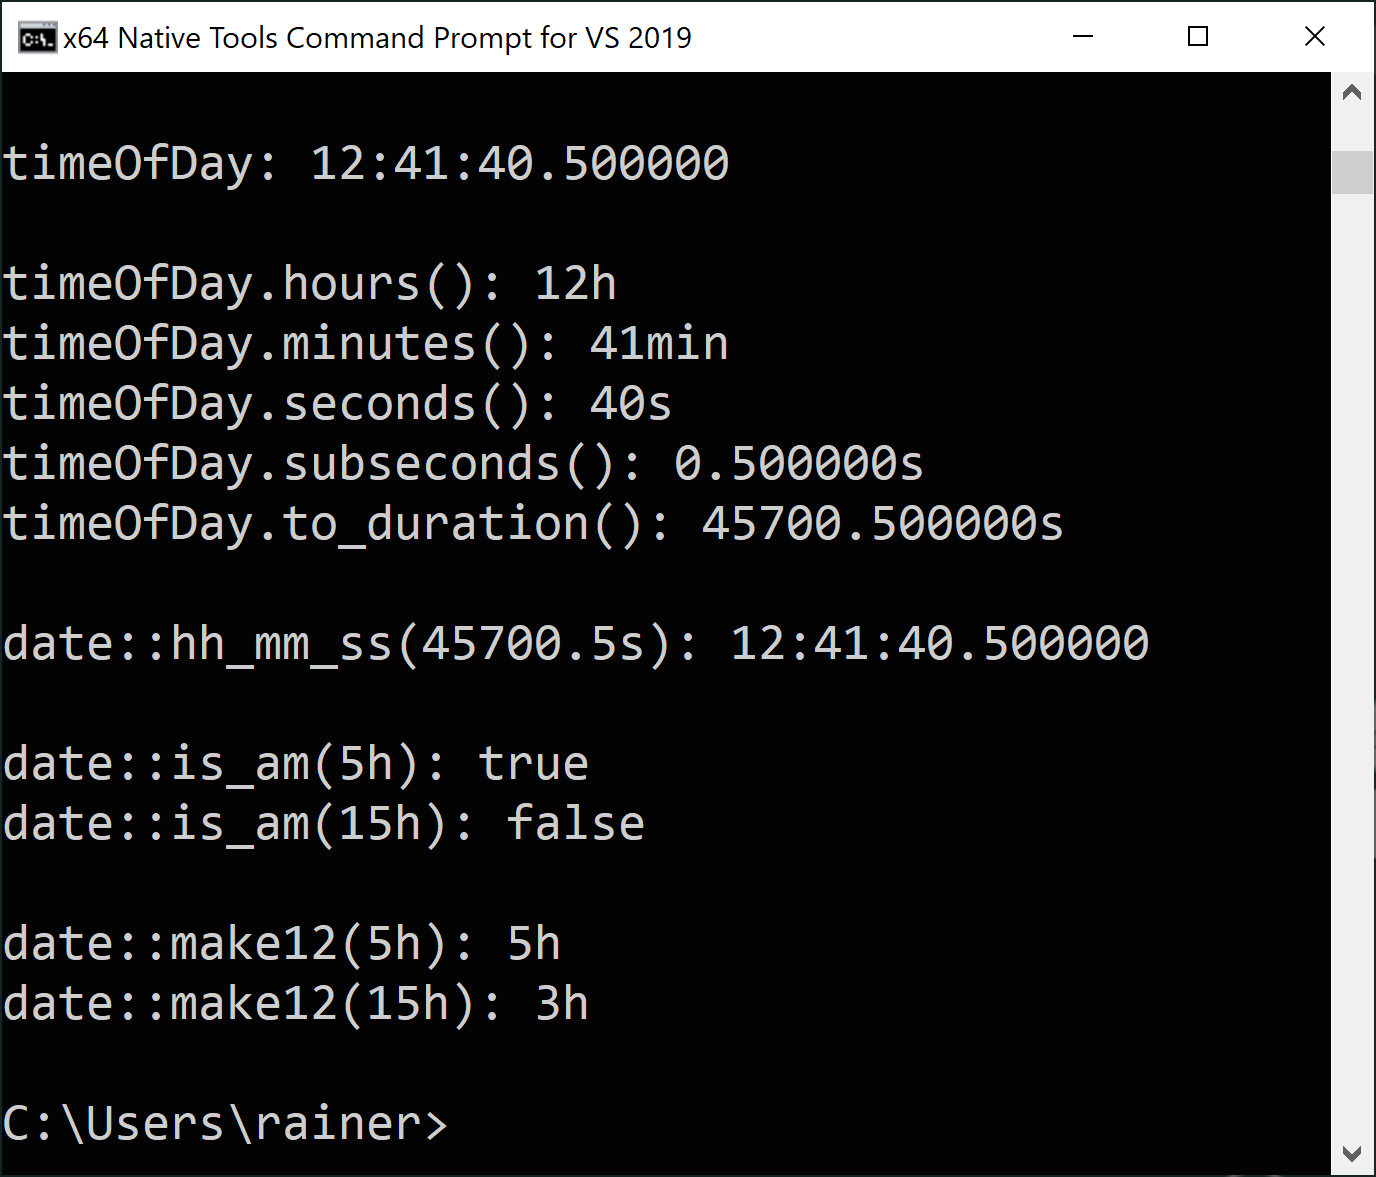
\includegraphics[width=0.6\textwidth]{content/3/chapter5/images/19.png}\\
Time of day
\end{center}


\subsubsubsection{5.5.2\hspace{0.2cm} Calendar Dates}

A new type of the chrono extension in C++20 is a calendar date. C++20 supports various ways to create a calendar date and interact with them. First of all: What is a calendar date?

A calendar date is a date that consists of a year, a month and a day. Consequently, C++20 has a specific data type std::chrono::year\_month\_day. C++20 has way more to offer. The following table should give you the first overview of calendar-date types before I show you various usecases.

\begin{center}
Various calendar-date types
\end{center}

\begin{table}[H]
\centering
\begin{tabular}{ll}
\textbf{Type}                 & \textbf{Description}                                   \\ \hline
std::chrono::last\_spec       & Indicates the last day or weekday of a month           \\
std::chrono::day              & Represents a day of a month                            \\
std::chrono::month            & Represents a month of a year                           \\
std::chrono::year             & Represents a year in the Gregorian calendar            \\
std::chrono::weekday          & Represents a day of the week in the Gregorian calendar \\
std::chrono::weekday\_indexed & Represents the n-th weekday of a month                 \\
std::chrono::weekday\_last    & Represents the last weekday of a month                 \\
std::chrono::month\_day       & Represents a specific day of a specific month          \\
std::chrono::month\_day\_last & Represents the last day of a specific month            \\
std::chrono::month\_weekday   & Represents the n-th weekday of a specific month        \\
std::chrono::month\_weekday\_last            & Represents the last weekday of a specific month           \\
std::chrono::year\_month      & Represents a specific month of a specific year         \\
std::chrono::year\_month\_day & Represents a specific year, month, and day             \\
std::chrono::year\_month\_day\_last          & Represents the last day of a specific year and month      \\
std::chrono::year\_month\_weekday            & Represents the n-th weekday of a specific year and month  \\
std::chrono::year\_month\_day\_weekday\_last & Represents the last weekday of a specific years and month \\
std::chrono::operator /       & Creates a date of the Gregorian calendar              
\end{tabular}
\end{table}

Let me start simple and create a few calendar dates.

\hspace*{\fill} \\ %插入空行
\noindent
\textbf{5.5.2.1\hspace{0.2cm} Create Calendar Dates}

The program createCalendar.cpp shows various ways to create calendar-related dates.

\hspace*{\fill} \\ %插入空行
\noindent
Create calendar dates
\begin{lstlisting}[style=styleCXX]
// createCalendar.cpp

#include <iostream>
#include "date.h"

int main() {

	std::cout << '\n';
	
	using namespace date;
	
	constexpr auto yearMonthDay{year(1940)/month(6)/day(26)};
	std::cout << yearMonthDay << " ";
	std::cout << date::year_month_day(1940_y, June, 26_d) << '\n';
	
	std::cout << '\n';
	
	constexpr auto yearMonthDayLast{year(2010)/March/last};
	std::cout << yearMonthDayLast << " ";
	std::cout << date::year_month_day_last(2010_y, month_day_last(month(3))) << '\n';
	
	constexpr auto yearMonthWeekday{year(2020)/March/Thursday[2]};
	std::cout << yearMonthWeekday << " ";
	std::cout << date::year_month_weekday(2020_y, month(March), Thursday[2]) << '\n';
	
	constexpr auto yearMonthWeekdayLast{year(2010)/March/Monday[last]};
	std::cout << yearMonthWeekdayLast << " ";
	std::cout << date::year_month_weekday_last(2010_y, month(March),
	weekday_last(Monday)) << '\n';
	
	std::cout << '\n';
	
	constexpr auto day_{day(19)};
	std::cout << day_ << " ";
	std::cout << date::day(19) << '\n';
	
	constexpr auto month_{month(1)};
	std::cout << month_ << " ";
	std::cout << date::month(1) << '\n';
	
	constexpr auto year_{year(1988)};
	std::cout << year_ << " ";
	std::cout << date::year(1988) << '\n';
	
	constexpr auto weekday_{weekday(5)};
	std::cout << weekday_ << " ";
	std::cout << date::weekday(5) << '\n';
	
	constexpr auto yearMonth{year(1988)/1};
	std::cout << yearMonth << " ";
	std::cout << date::year_month(year(1988), January) << '\n';
	
	constexpr auto monthDay{10/day(22)};
	std::cout << monthDay << " ";
	std::cout << date::month_day(October, day(22)) << '\n';
	
	constexpr auto monthDayLast{June/last};
	std::cout << monthDayLast << " ";
	std::cout << date::month_day_last(month(6)) << '\n';
	
	constexpr auto monthWeekday{2/Monday[3]};
	std::cout << monthWeekday << " ";
	std::cout << date::month_weekday(February, Monday[3]) << '\n';
	
	constexpr auto monthWeekDayLast{June/Sunday[last]};
	std::cout << monthWeekDayLast << " ";
	std::cout << date::month_weekday_last(June, weekday_last(Sunday)) << '\n';
	
	std::cout << '\n';

}
\end{lstlisting}

There are essentially two ways to create a calendar date. You can use the so-called cute syntax yearMonthDay\{year(1940)/month(6)/day(26)\} (line 12), or you can use the explicit type date::year\_month\_day(1940y, June, 26d) (line 14). In order not to overwhelm you, I will delay my explanation of the cute syntax to the next section. The explicit type is quite interesting, because it uses the date-time literals 1940y, 26d, and the predefined constant June. This was the obvious part of the program.

Line 18, line 22, and line 26 offer further ways to create calendar dates.

\begin{enumerate}
\item 
Line 18: the last day of March 2010: 
\begin{lstlisting}[style=styleCXX]
{year(2010)/March/last}
\end{lstlisting}
or
\begin{lstlisting}[style=styleCXX]
year_month_day_last(2010y, month_day_last(month(3)))
\end{lstlisting}

\item 
Line 22: the second Thursday of March 2020:
\begin{lstlisting}[style=styleCXX]
{year(2020)/March/Thursday[2]}
\end{lstlisting}
or
\begin{lstlisting}[style=styleCXX]
year_month_weekday(2020y, month(March), Thursday[2])
\end{lstlisting}

\item 
Line 26: the last Monday of March 2010: 
\begin{lstlisting}[style=styleCXX]
{year(2010)/March/Monday[last]}
\end{lstlisting}
or
\begin{lstlisting}[style=styleCXX]
year_month_weekday_last(2010y, month(March), weekday_last(Monday))
\end{lstlisting}
\end{enumerate}

The remaining calendar types stand for a day (line 33), a month (line 37), or a year (line 41). You can combine and use them as basic building blocks for fully specified calendar dates, such as in lines 18, 22, or 26.

This is the output of the program:

\begin{center}
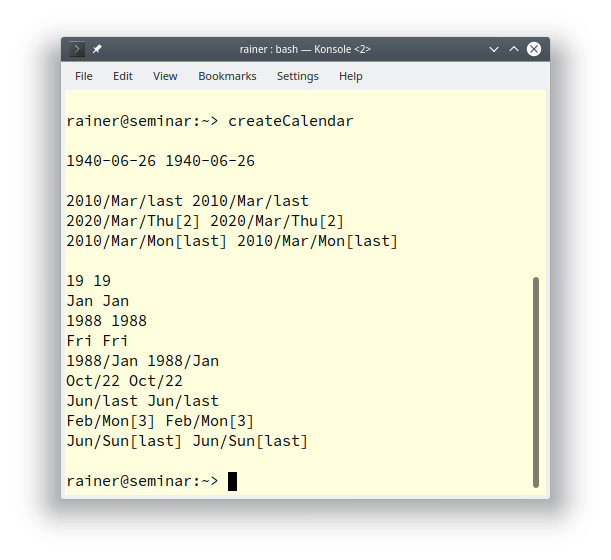
\includegraphics[width=0.6\textwidth]{content/3/chapter5/images/20.png}\\
Various calendar days
\end{center}

As promised, let me write about the cute syntax.

\hspace*{\fill} \\ %插入空行
\noindent
\textbf{5.5.2.2\hspace{0.2cm} Cute Syntax}

The cute syntax consists of overloaded division operators to specify a calendar date. The overloaded operators support time literals (e.g.: 2020y, 31d) and constants (January, February, March, April, May, June, July, August, September, October, November, December).

The following three combinations of year, month, and day are possible when you use the cute syntax.

\hspace*{\fill} \\ %插入空行
\noindent
Cute syntax
\begin{lstlisting}[style=styleCXX]
year/month/day
day/month/year
month/day/year
\end{lstlisting}

These combinations are not arbitrarily chosen. They are the ones used worldwide. Any other combination is not allowed.

Consequently, when you choose the type year, month, or day for the first argument, the type for the remaining two arguments is no longer necessary anymore, and a number would do the job.

\hspace*{\fill} \\ %插入空行
\noindent
Cute syntax
\begin{lstlisting}[style=styleCXX]
// cuteSyntax.cpp

#include <iostream>
#include "date.h"

int main() {
	
	std::cout << '\n';
	
	using namespace date;
	
	constexpr auto yearMonthDay{year(1966)/6/26};
	std::cout << yearMonthDay << '\n';
	
	constexpr auto dayMonthYear{day(26)/6/1966};
	std::cout << dayMonthYear << '\n';
	
	constexpr auto monthDayYear{month(6)/26/1966};
	std::cout << monthDayYear << '\n';
	
	constexpr auto yearDayMonth{year(1966)/month(26)/6};
	std::cout << yearDayMonth << '\n';
	
	std::cout << '\n';

}
\end{lstlisting}

The combination year/day/month (line 21) is not allowed and causes a run-time message.

\begin{center}
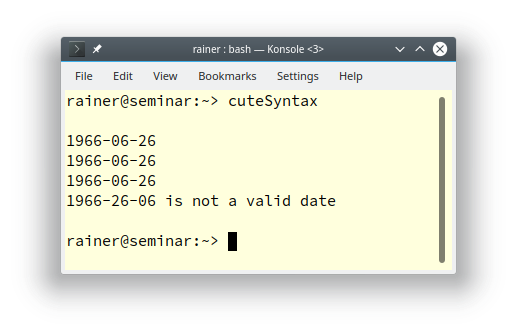
\includegraphics[width=0.6\textwidth]{content/3/chapter5/images/21.png}\\
Use of cute syntax
\end{center}

I assume you want to display a calendar date \{year(2010)/March/last\} in a readable form, for example, 2020-03-31. This is a job for the local\_days or sys\_days operator.

\hspace*{\fill} \\ %插入空行
\noindent
\textbf{5.5.2.3\hspace{0.2cm} Displaying Calendar Dates}

Thanks to std::chrono::local\_days or std::chrono::sys\_days, you can convert calendar dates to a std::chrono::time\_point. I use std::chrono::sys\_days in my example. std::chrono::sys\_days is based on \href{https://en.cppreference.com/w/cpp/chrono/system_clock}{std::chrono::system\_clock}. Let me convert the calendar dates (lines 18, 22, and 26) from the previous program createCalendar.cpp.

\hspace*{\fill} \\ %插入空行
\noindent
Displaying calendar dates
\begin{lstlisting}[style=styleCXX]
 // sysDays.cpp

#include <iostream>
#include "date.h"

int main() {

	std::cout << '\n';
	
	using namespace date;
	
	constexpr auto yearMonthDayLast{year(2010)/March/last};
	std::cout << "sys_days(yearMonthDayLast): "
	<< sys_days(yearMonthDayLast) << '\n';
	
	constexpr auto yearMonthWeekday{year(2020)/March/Thursday[2]};
	std::cout << "sys_days(yearMonthWeekday): "
	<< sys_days(yearMonthWeekday) << '\n';
	
	constexpr auto yearMonthWeekdayLast{year(2010)/March/Monday[last]};
	std::cout << "sys_days(yearMonthWeekdayLast): "
	<< sys_days(yearMonthWeekdayLast) << '\n';
	
	std::cout << '\n';
	
	constexpr auto leapDate{year(2012)/February/last};
	std::cout << "sys_days(leapDate): " << sys_days(leapDate) << '\n';
	
	constexpr auto noLeapDate{year(2013)/February/last};
	std::cout << "sys_day(noLeapDate): " << sys_days(noLeapDate) << '\n';
	
	std::cout << '\n';

}
\end{lstlisting}

The std::chrono::last constant (line 11) lets me easily determine how many days a month has. The output shows that 2012 is a leap year (line 26), but not 2013 (line 29).

\begin{center}
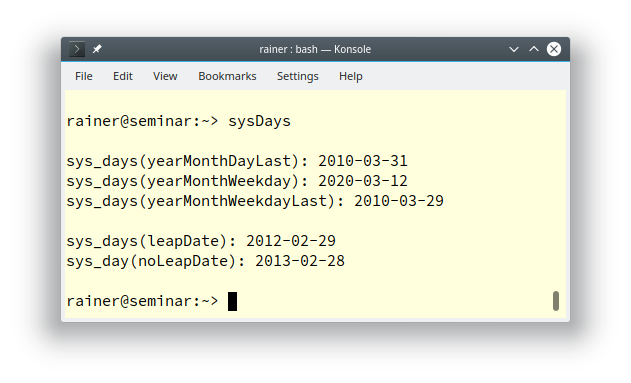
\includegraphics[width=0.6\textwidth]{content/3/chapter5/images/22.png}\\
Displaying calendar dates
\end{center}

Assume you have a calendar date such as year(2100)/2/29. Your first question may be: Is this date valid?

\hspace*{\fill} \\ %插入空行
\noindent
\textbf{5.5.2.4\hspace{0.2cm} Check if a Date is valid}

The various calendar types in C++20 have a function ok. This function returns true if the date is valid.

\hspace*{\fill} \\ %插入空行
\noindent
Checking if a date is valid
\begin{lstlisting}[style=styleCXX]
// leapYear.cpp

#include <iostream>
#include "date.h"

int main() {
	
	std::cout << std::boolalpha << '\n';
	
	using namespace date;
	
	std::cout << "Valid days" << '\n';
	day day31(31);
	day day32 = day31 + days(1);
	std::cout << " day31: " << day31 << "; ";
	std::cout << "day31.ok(): " << day31.ok() << '\n';
	std::cout << " day32: " << day32 << "; ";
	std::cout << "day32.ok(): " << day32.ok() << '\n';
	
	
	std::cout << '\n';
	
	std::cout << "Valid months" << '\n';
	month month1(1);
	month month0(0);
	std::cout << " month1: " << month1 << "; ";
	std::cout << "month1.ok(): " << month1.ok() << '\n';
	std::cout << " month0: " << month0 << "; ";
	std::cout << "month0.ok(): " << month0.ok() << '\n';
	
	std::cout << '\n';
	
	std::cout << "Valid years" << '\n';
	year year2020(2020);
	year year32768(-32768);
	std::cout << " year2020: " << year2020 << "; ";
	std::cout << "year2020.ok(): " << year2020.ok() << '\n';
	std::cout << " year32768: " << year32768 << "; ";
	std::cout << "year32768.ok(): " << year32768.ok() << '\n';
	
	std::cout << '\n';
	
	std::cout << "Leap Years" << '\n';
	
	constexpr auto leapYear2016{year(2016)/2/29};
	constexpr auto leapYear2020{year(2020)/2/29};
	constexpr auto leapYear2024{year(2024)/2/29};
	
	std::cout << " leapYear2016.ok(): " << leapYear2016.ok() << '\n';
	std::cout << " leapYear2020.ok(): " << leapYear2020.ok() << '\n';
	std::cout << " leapYear2024.ok(): " << leapYear2024.ok() << '\n';
	
	std::cout << '\n';
	
	std::cout << "No Leap Years" << '\n';
	
	constexpr auto leapYear2100{year(2100)/2/29};
	constexpr auto leapYear2200{year(2200)/2/29};
	constexpr auto leapYear2300{year(2300)/2/29};
	
	std::cout << " leapYear2100.ok(): " << leapYear2100.ok() << '\n';
	std::cout << " leapYear2200.ok(): " << leapYear2200.ok() << '\n';
	std::cout << " leapYear2300.ok(): " << leapYear2300.ok() << '\n';
	
	std::cout << '\n';
	
	std::cout << "Leap Years" << '\n';
	
	constexpr auto leapYear2000{year(2000)/2/29};
	constexpr auto leapYear2400{year(2400)/2/29};
	constexpr auto leapYear2800{year(2800)/2/29};
	
	std::cout << " leapYear2000.ok(): " << leapYear2000.ok() << '\n';
	std::cout << " leapYear2400.ok(): " << leapYear2400.ok() << '\n';
	std::cout << " leapYear2800.ok(): " << leapYear2800.ok() << '\n';
	
	std::cout << '\n';

}
\end{lstlisting}

I check in the program if a given day (line 12), a given month (line 23), or a given year (line 33) is valid. The range of a day is [1, 31], of a month [1, 12], and of a year [ -32767, 32767]. Consequently, the ok() calls on the corresponding values returns false. Two facts are interesting when I display various values. First, if the value is not valid, the output displays: “is not a valid day”, “is not a valid month”, “is not a valid year”. Second, month values are displayed in string representation.

\begin{center}
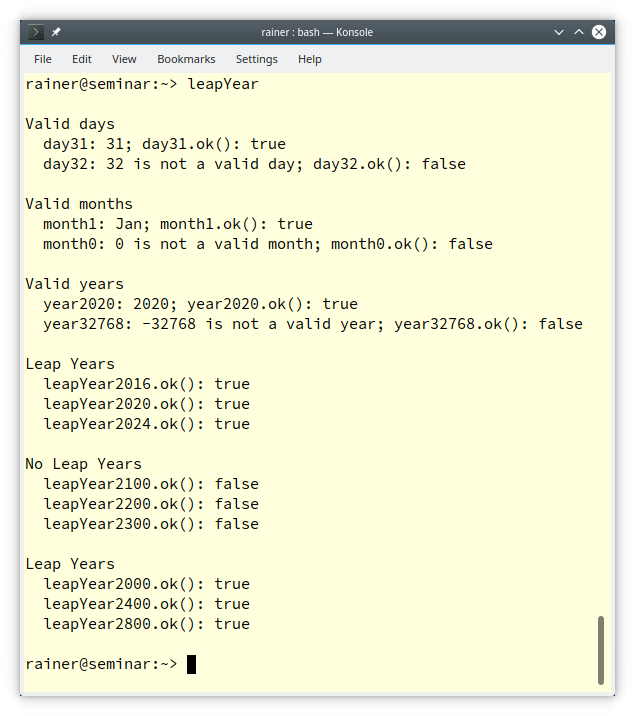
\includegraphics[width=0.6\textwidth]{content/3/chapter5/images/23.png}\\
Check if a data is valid
\end{center}

You can apply the ok-call on a calendar date. Now it’s quite easy to check if a specific calendar date is a leap day and, therefore, the corresponding year a leap year. In the worldwide used \href{https://en.wikipedia.org/wiki/Gregorian_calendar}{Gregorian calendar}, the following rules apply:

Each year that is exactly divisible by 4 is a leap year.
 
\begin{itemize}
\item 
Except for years which are exactly divisible by 100. They are not leap years.

\begin{itemize}
\item 
Except for years which are exactly divisible by 400. They are leap years.
\end{itemize}
\end{itemize}

Too complicated? The program leapYears.cpp exemplifies this rule.

The extended chrono library makes it quite easy to ask for the time duration between calendar dates.

\hspace*{\fill} \\ %插入空行
\noindent
\textbf{5.5.2.5\hspace{0.2cm} Query Calendar Dates}

Without further ado. The following program queryCalendarDates.cpp queries a few calendar dates.

\hspace*{\fill} \\ %插入空行
\noindent
Query calendar dates
\begin{lstlisting}[style=styleCXX]
// queryCalendarDates.cpp

#include "date.h"
#include <iostream>

int main() {
	
	using namespace date;
	
	std::cout << '\n';
	
	auto now = std::chrono::system_clock::now();
	std::cout << "The current time is: " << now << " UTC\n";
	std::cout << "The current date is: " << floor<days>(now) << '\n';
	std::cout << "The current date is: " << year_month_day{floor<days>(now)}
	<< '\n';
	std::cout << "The current date is: " << year_month_weekday{floor<days>(now)}
	<< '\n';
	
	std::cout << '\n';
	
	
	auto currentDate = year_month_day(floor<days>(now));
	auto currentYear = currentDate.year();
	std::cout << "The current year is " << currentYear << '\n';
	auto currentMonth = currentDate.month();
	std::cout << "The current month is " << currentMonth << '\n';
	auto currentDay = currentDate.day();
	std::cout << "The current day is " << currentDay << '\n';
	
	std::cout << '\n';
	
	auto hAfter = floor<std::chrono::hours>(now) - sys_days(January/1/currentYear);
	std::cout << "It has been " << hAfter << " since New Year!\n";
	
	auto nextYear = currentDate.year() + years(1);
	auto nextNewYear = sys_days(January/1/nextYear);
	auto hBefore = sys_days(January/1/nextYear) - floor<std::chrono::hours>(now);
	std::cout << "It is " << hBefore << " before New Year!\n";
	
	std::cout << '\n';
	
	std::cout << "It has been " << floor<days>(hAfter) << " since New Year!\n";
	std::cout << "It is " << floor<days>(hBefore) << " before New Year!\n";
	
	std::cout << '\n';
	
}
\end{lstlisting}

With the C++20 extension, you can directly display a time point, such as now (line 12). std::chrono::floor converts the time point to a day std::chrono::sys\_days. This value can be used to initialize the calendar type std::chrono::year\_month\_day. Finally, when I put the value into a std::chrono::year\_month\_weekday calendar type, I get the answer that this specific day is the 3rd Tuesday in October. Of course, I can also ask a calendar date for its components, such as the current year, month, or day (line 23).

Line 33 is the most interesting one. When I subtract from the current date, using hour resolution, the first of January of the current year, I get the number of hours since the new year. Conversely, when I subtract from the first of January of the next year (line 37) the current date, using hour resolution, I get the hours to the new year. Maybe you don’t like hour resolution. Line 42 and 43 display the values using day resolution.

\begin{center}
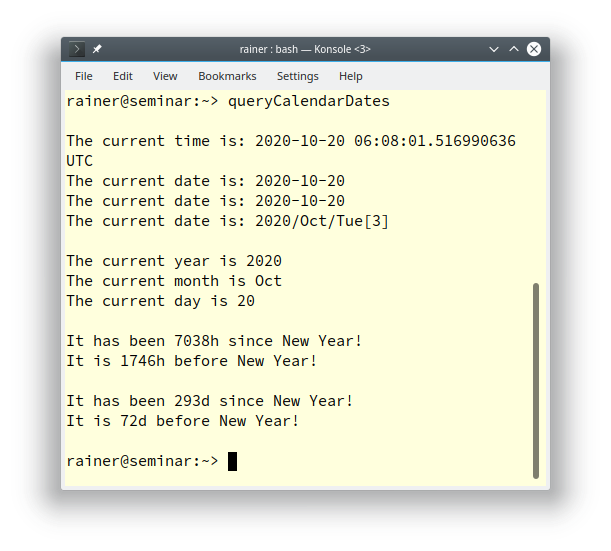
\includegraphics[width=0.6\textwidth]{content/3/chapter5/images/24.png}\\
Query calendar days
\end{center}

Now, I want to know the day of the week of my birthday.

\hspace*{\fill} \\ %插入空行
\noindent
\textbf{5.5.2.6\hspace{0.2cm} Query Weekdays}

Thanks to the extended chrono library, it is quite easy to get the weekday of a given calendar date.

\hspace*{\fill} \\ %插入空行
\noindent
Weekdays of given calendar dates
\begin{lstlisting}[style=styleCXX]
// weekdaysOfBirthdays.cpp

#include <cstdlib>
#include <iostream>
#include "date.h"

int main() {
	
	std::cout << '\n';
	
	using namespace date;
	
	int y;
	int m;
	int d;
	
	std::cout << "Year: ";
	std::cin >> y;
	std::cout << "Month: ";
	std::cin >> m;
	std::cout << "Day: ";
	std::cin >> d;
	
	std::cout << '\n';
	
	auto birthday = year(y)/month(m)/day(d);
	
	if (not birthday.ok()) {
		std::cout << birthday << '\n';
		std::exit(EXIT_FAILURE);
	}
	
	std::cout << "Birthday: " << birthday << '\n';
	auto birthdayWeekday = year_month_weekday(birthday);
	std::cout << "Weekday of birthday: " << birthdayWeekday.weekday() << '\n';
	
	auto currentDate = year_month_day(floor<days>(
	std::chrono::system_clock::now()));
	auto currentYear = currentDate.year();
	
	auto age = (int)currentDate.year() - (int)birthday.year();
	std::cout << "Your age: " << age << '\n';
	
	std::cout << '\n';
	
	std::cout << "Weekdays for your next 10 birthdays" << '\n';
	
	for (int i = 1, newYear = (int)currentYear; i <= 10; ++i ) {
		std::cout << " Age " << ++age << '\n';
		auto newBirthday = year(++newYear)/month(m)/day(d);
		std::cout << " Birthday: " << newBirthday << '\n';
		std::cout << " Weekday of birthday: "
				  << year_month_weekday(newBirthday).weekday() << '\n';
	}
	
	std::cout << '\n';
	
}
\end{lstlisting}

First, the program asks you for the year, month, and day of your birthday (line 17). Based on the input, a calendar date is created (line 26) and checked if it’s valid (line 28). Now I display the weekday of your birthday. I use the calendar date to fill the calendar type std::chrono::year\_month\_weekday (line 34). To get the int representation of the calendar type year, I have to convert it to int (line 41). Now I can display your age. Finally, the for loop displays, for each of your next ten birthdays (line 46), the following information: your age, the calendar date, and the weekday. I just have to increment the age and newYear variable.

Here is a run of the program with my birthday.

\begin{center}
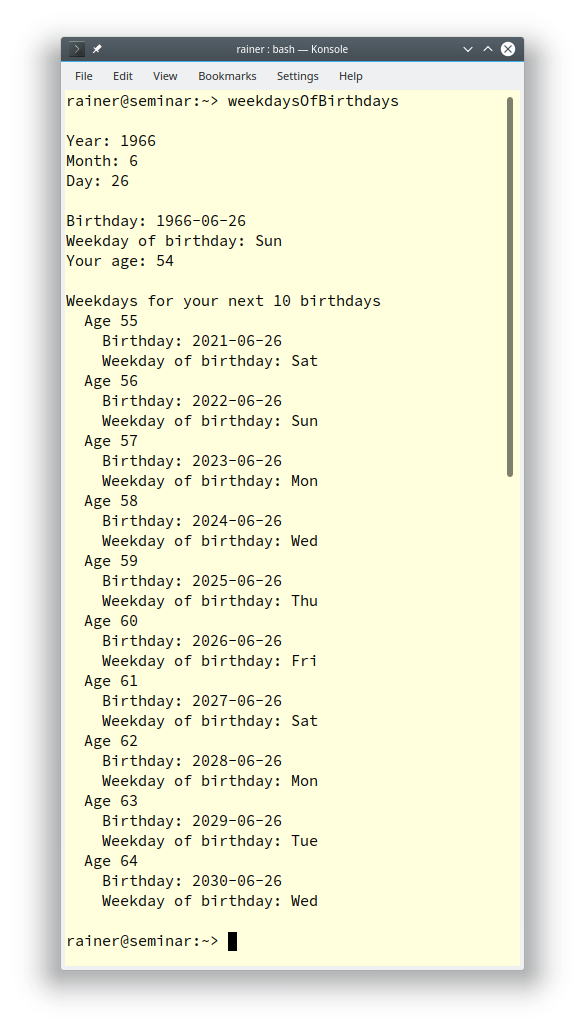
\includegraphics[width=0.6\textwidth]{content/3/chapter5/images/25.png}\\
Weekdays of birthdays
\end{center}

\hspace*{\fill} \\ %插入空行
\noindent
\textbf{5.5.2.7\hspace{0.2cm} Calculating Ordinal Dates}

As a last example of the new calendar facility, I want to present the online resource \href{https://github.com/HowardHinnant/date/wiki/Examples-and-Recipes}{Examples and Recipes} from Howard Hinnant, which has about 40 examples of the new chrono functionality. Presumably, the chrono extension in C++20 is not easy to get, therefore it’s quite important to have so many examples. You should use these examples as a starting point for further experiments and, therefore, sharpen your understanding. You can also add your recipes.

To get an idea of Examples and Recipes I want to present a program by \href{https://github.com/rbock}{Roland Bock} that calculates ordinal dates.

“An ordinal date consists of a year and a day of year (1st of January being day 1, 31st of December being day 365 or day 366). The year can be obtained directly from year\_month\_day. And calculating the day is wonderfully easy. In the code below we make us of the fact that year\_month\_day can deal with invalid dates like the 0th of January:” (Roland Bock) I added the necessary headers to Roland’s program.

\hspace*{\fill} \\ %插入空行
\noindent
Calculating ordinal dates
\begin{lstlisting}[style=styleCXX]
// ordinalDate.cpp

#include "date.h"
#include <iomanip>
#include <iostream>

int main()
{
	using namespace date;
	
	const auto time = std::chrono::system_clock::now();
	const auto daypoint = floor<days>(time);
	const auto ymd = year_month_day{daypoint};
	
	// calculating the year and the day of the year
	const auto year = ymd.year();
	const auto year_day = daypoint - sys_days{year/January/0};
	
	std::cout << year << '-' << std::setfill('0') << std::setw(3)
	          << year_day.count() << '\n';
	
	// inverse calculation and check
	assert(ymd == year_month_day{sys_days{year/January/0} + year_day});
}
\end{lstlisting}

I want to make a few remarks about the program. Line 12 truncates the current time point. The value is used in the following line to initialize a calendar date. Line 17 calculates the time duration between the two time points. Both time points have the resolution day. Finally, year\_day.count() in line 19 returns the time duration in days.

\begin{center}
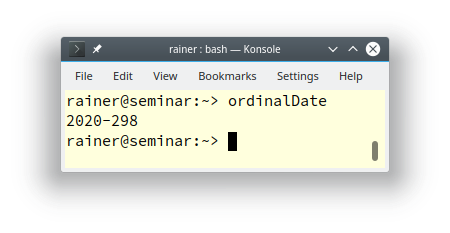
\includegraphics[width=0.6\textwidth]{content/3/chapter5/images/26.png}\\
Caculating ordinal dates
\end{center}

\subsubsubsection{5.5.3\hspace{0.2cm} Time Zones}

First of all, a time zone is a region, and its full history of the date, such as daylight saving time or leap seconds. The time zone library in C++20 is a complete parser of the \href{https://www.iana.org/timezones}{IANA timezone database}. The following table should give you a first idea of the new functionality.

\begin{center}
The time-zone data types
\end{center}

\begin{table}[H]
\centering
\begin{tabular}{ll}
\textbf{Type}                         & \textbf{Description}                                              \\ \hline
std::chrono::tzdb                     & Describes a copy of the IANA time-zone database                   \\
std::chrono::tdzb\_list               & Represents a linked list of the tzdb                              \\
\begin{tabular}[c]{@{}l@{}}std::chrono::get\_tzdb \\ std::chrono::get\_tzdb\_list \\ std::chrono::reload\_tzdb \\ std::chrono::remote\_version\end{tabular} &
Accesses and controls the global time-zone database \\
std::chrono::locate\_zone             & Locates the time zone based on its name                           \\
std::chrono::current\_zone            & Returns the current time zone                                     \\
std::chrono::time\_zone               & Represents a time zone                                            \\
std::chrono::sys\_info                & Represents information about a time zone at a specific time point \\
std::chrono::local\_info              & Represents information about a local time to UNIX time conversion \\
std::chrono::zoned\_traits            & Class for time zone pointers                                      \\
std::chrono::zoned\_time              & Represents a time zone and a time point                           \\
std::chrono::leap\_second             & Contains information about a leap-second insertion                \\
std::chrono::time\_zone\_link         & Represents an alternative name for a time zone                    \\
std::chrono::nonexistent\_local\_time & Exception which is thrown if a local time does not exist         
\end{tabular}
\end{table}

I use in my examples the function std::chrono::zones\_time, which is essentially a time zone combined with a time point.

\begin{tcolorbox}[colback=blue!5!white,colframe=blue!75!black,title={Compilation of the examples}]
	
Before I show you two examples, I want to make a short remark. To compile a program using the time zone library, you have to compile the tz.cpp file from the \href{https://github.com/HowardHinnant/date}{date} library and link it against the \href{https://curl.se/}{curl} library. The curl library is necessary to get the current \href{https://www.iana.org/timezones}{IANA timezone database}. The following command line for g++ should give you the idea:

\hspace*{\fill} \\ %插入空行
\noindent
Compilation with the prototype library date
\begin{tcblisting}{commandshell={}}
g++ localTime.cpp -I <Path to data/tz.h> tz.cpp -std=c++17 \
  -lcurl -o localTime
\end{tcblisting}

\end{tcolorbox}

My first example is straightforward. It displays the UTC time and the local time.

\hspace*{\fill} \\ %插入空行
\noindent
\textbf{5.5.3.1\hspace{0.2cm} UTC Time and Local Time}

The \href{https://en.wikipedia.org/wiki/Coordinated_Universal_Time}{UTC time or Coordinated Universal Time} is the primary time standard worldwide. A computer uses \href{https://en.wikipedia.org/wiki/Unix_time}{Unix time} which is a very close approximation of UTC. The UNIX time is the number of seconds since the Unix epoch. The Unix epoch is 00:00:00 UTC on 1 January 1970.

std::chrono::system\_clock::now() returns in the program localTime.cpp the Unix time.

\hspace*{\fill} \\ %插入空行
\noindent
Getting the UTC time and local time
\begin{lstlisting}[style=styleCXX]
// localTime.cpp

#include "date/tz.h"
#include <iostream>

int main() {

	std::cout << '\n';
	
	using namespace date;
	
	std::cout << "UTC time" << '\n';
	auto utcTime = std::chrono::system_clock::now();
	std::cout << " " << utcTime << '\n';
	std::cout << " " << date::floor<std::chrono::seconds>(utcTime) << '\n':
	
	std::cout << '\n';
	
	std::cout << "Local time" << '\n';
	auto localTime = date::make_zoned(date::current_zone(), utcTime);
	std::cout << " " << localTime << '\n';
	std::cout << " " << date::floor<std::chrono::seconds>(localTime.get_local_time())
	          << '\n';
	
	auto offset = localTime.get_info().offset;
	std::cout << " UTC offset: " << offset << '\n';

	std::cout << '\n';

}
\end{lstlisting}

The code block beginning with line 12 gets the current time point, truncates it to seconds, and displays it. The call make\_zoned (line 20) creates a std::chrono::zoned\_time localTime. After that, the call localTime.get\_local\_time() returns the stored time point as a local time. This time point is also truncated to seconds. localTime (line 25) can also be used to get information about the time zone. In this case, I’m interested in the offset to the UTC time.

\begin{center}
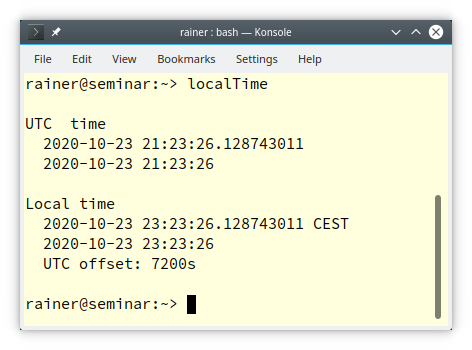
\includegraphics[width=0.6\textwidth]{content/3/chapter5/images/27.png}\\
Displaying UTC time and local time
\end{center}

My last example answers a crucial question when I teach in a different time zone: When should I start my online class?

\hspace*{\fill} \\ %插入空行
\noindent
\textbf{5.5.3.2\hspace{0.2cm} Various Time Zones for Online Classes}

The program onlineClass.cpp answers the following question: How late is it in given time zones, when I start an online class at the 7h, 13h, or 17h local time (Germany)?

The online class should start on the 1st of February 2021 and should take four hours. Because of daylight saving time, the calendar date is essential to get the correct answer.

\hspace*{\fill} \\ %插入空行
\noindent
Calculating the time in different time zones
\begin{lstlisting}[style=styleCXX]
// onlineClass.cpp

#include "date/tz.h"
#include <algorithm>
#include <iomanip>
#include <iostream>

template <typename ZonedTime>
auto getMinutes(const ZonedTime& zonedTime) {
	return date::floor<std::chrono::minutes>(zonedTime.get_local_time());
}

void printStartEndTimes(const date::local_days& localDay,
						const std::chrono::hours& h,
						const std::chrono::hours& durationClass,
						const std::initializer_list<std::string>& timeZones ){
	
	date::zoned_time startDate{date::current_zone(), localDay + h};
	date::zoned_time endDate{date::current_zone(), localDay + h + durationClass};
	std::cout << "Local time: [" << getMinutes(startDate) << ", "
	<< getMinutes(endDate) << "]" << '\n';
	
	longestStringSize = std::max(timeZones, [](const std::string& a,
	const std::string& b) { return a.size() < b.size(); }).size();
	for (auto timeZone: timeZones) {
		std::cout << " " << std::setw(longestStringSize + 1) << std::left
		          << timeZone
		          << "[" << getMinutes(date::zoned_time(timeZone, startDate))
		          << ", " << getMinutes(date::zoned_time(timeZone, endDate))
		          << "]" << '\n';
		
	}
}

int main() {

	using namespace std::string_literals;
	using namespace std::chrono;
	
	std::cout << '\n';
	
	constexpr auto classDay{date::year(2021)/2/1};
	constexpr auto durationClass = 4h;
	auto timeZones = {"America/Los_Angeles"s, "America/Denver"s,
					  "America/New_York"s, "Europe/London"s,
					  "Europe/Minsk"s, "Europe/Moscow"s,
					  "Asia/Kolkata"s, "Asia/Novosibirsk"s,
					  "Asia/Singapore"s, "Australia/Perth"s,
					  "Australia/Sydney"s};
	
	for (auto startTime: {7h, 13h, 17h}) {
		printStartEndTimes(date::local_days{classDay}, startTime,
						   durationClass, timeZones);
		std::cout << '\n';
	}

}
\end{lstlisting}

Before I dive into the functions getMinutes (line 8) and printStartEndTimes (line 13), let me say a few words about the main function. The main function defines the day of the class, the duration of the class, and all time zones. Finally, the range-based for loop (line 51) iterates through all potential starting points for an online class. Thanks to the function printStartEndTimes (line 13), all necessary information is displayed.

The few lines beginning with line 18 calculate the startDate and endDate of my training by adding the start time and the duration of the class to the calendar date. Both values are displayed with the help of the function getMinutes (line 8). floor<std::chrono::minutes>(zonedTime.get\_local\_time()) gets the stored timepoint out of the std::chrono::zoned\_time and truncates the value to the minute resolution. To properly align the output of the program, line 23 determines the size of the longest of all timezone names. Line 25 iterates through all time zones and displays the name of the time zone, and the beginning and end of each online class. A few calendar dates even cross the day boundaries.

\begin{center}
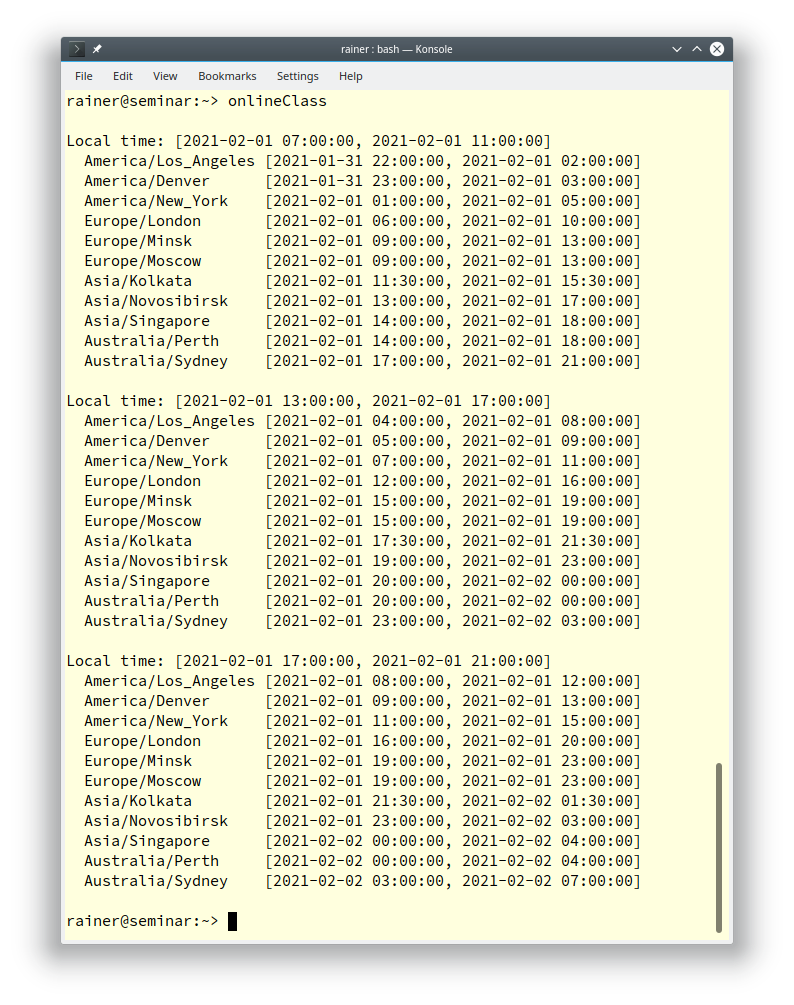
\includegraphics[width=0.6\textwidth]{content/3/chapter5/images/28.png}\\
Displaying start and end times in various time zones
\end{center}


\hspace*{\fill} \\ %插入空行
\noindent
\textbf{5.5.3.3\hspace{0.2cm} New Clocks}

Beside the wall clock \href{https://www.modernescpp.com/index.php/the-three-clocks}{std::system\_clock}, the monotonic clock std::steady\_clock, and the most precise clock std::high\_resolution\_clock in C++11, C++20 supports five additional clocks.

\begin{itemize}
\item 
std::utc\_clock: Clock for the coordinated Universal Time (UTC). Measures the time since 00:00:00 UTC, 1 January 1970, including leap seconds.

\item 
std::tai\_clock: Clock for \href{https://en.wikipedia.org/wiki/International_Atomic_Time}{International Atomic Time} (TAI). Measure time since 00:00:00, 1 January 1958, and is offset 10 seconds ahead of UTC at that date. Leap seconds are not inserted.

\item 
std::gps\_clock: Clock for GPS time. It represents \href{https://en.wikipedia.org/wiki/Global_Positioning_System}{Global Positioning System} (GPS) time. It measures the time since 00:00:00, 6 January 1980 UTC. Leap seconds are not inserted.

\item 
std::file\_clock: Clock for file time. It’s an alias for \href{https://en.cppreference.com/w/cpp/filesystem/file_time_type}{std::filesystem::file\_time\_type}.

\item 
std::local\_t: Pseudo clock to represent local time.
\end{itemize}


\hspace*{\fill} \\ %插入空行
\noindent
\textbf{5.5.3.4\hspace{0.2cm} Chrono I/O}

Thanks to the function std::chrono::parse and the std::formatter from the formatting library, you can read and write chrono objects.

\begin{itemize}
\item 
std::chrono::parse: Parses a chrono object from a stream. \href{https://en.cppreference.com/w/cpp/chrono/parse}{cppreference.com/parse} gives you detailed infomation about the format string.

\item 
std::formatter: Defines specializations for the various chrono types. Read the details on the format specification on std::formatter here \href{https://en.cppreference.com/w/cpp/chrono/system_clock/formatter#Format_specification}{cppreference.com/formatter}.
\end{itemize}

\begin{tcolorbox}[colback=mygreen!5!white,colframe=mygreen!75!black,title={Distilled Information}]

\begin{itemize}
\item 
C++20 adds new components to the chrono library: time of day, calendar, and time zone.

\item 
Time of day is the time duration since midnight, split into hours, minutes, seconds, and fractional seconds.

\item 
Calendar stands for various calendar dates such as year, a month, a weekday, or the n-th day of a week.

\item 
 A time zone represents time specific to a geographic area.
\end{itemize}

\end{tcolorbox}








